%%%%%%%%%%%%%%%%%%%%%%%%%%%%%%%%%%%%%%%%%%%%%%%%%%%%%%%%%%%%%%%%%%%%%
% LaTeX Template: Project Titlepage Modified (v 0.1) by rcx
%
% Original Source: http://www.howtotex.com
% Date: February 2014
% 
% This is a title page template which be used for articles & reports.
% 
% This is the modified version of the original Latex template from
% aforementioned website.
% 
%%%%%%%%%%%%%%%%%%%%%%%%%%%%%%%%%%%%%%%%%%%%%%%%%%%%%%%%%%%%%%%%%%%%%%

\documentclass[12pt]{report}
\usepackage[a4paper]{geometry}
\usepackage[myheadings]{fullpage}
\usepackage{fancyhdr}
\usepackage{lastpage}
\usepackage{graphicx, wrapfig, subcaption, setspace, booktabs}
\usepackage[T1]{fontenc}
\usepackage[font=small, labelfont=bf]{caption}
\usepackage{fourier}
\usepackage[protrusion=true, expansion=true]{microtype}
\usepackage[english]{babel}
\usepackage{sectsty}
\usepackage{url, lipsum}


\newcommand{\HRule}[1]{\rule{\linewidth}{#1}}
\onehalfspacing
\setcounter{tocdepth}{5}
\setcounter{secnumdepth}{5}

%-------------------------------------------------------------------------------
% HEADER & FOOTER
%-------------------------------------------------------------------------------
\pagestyle{fancy}
\fancyhf{}
\setlength\headheight{15pt}
\fancyhead[L]{Group 4}
\fancyhead[R]{SIAT Deep learning project}
\fancyfoot[R]{Page \thepage\ of \pageref{LastPage}}
%-------------------------------------------------------------------------------
% TITLE PAGE
%-------------------------------------------------------------------------------

\begin{document}

\title{ \normalsize \textsc{}
		\\ [2.0cm]
		\HRule{0.5pt} \\
		\LARGE \textbf{\uppercase{KNN Algorithm on Image recognition}}
		\HRule{2pt} \\ [0.5cm]
		\normalsize \today \vspace*{5\baselineskip}}

\date{}

\author{
		Group 4 \\ 
		\\
		Wang Kou, Chen Xinrui, Ji Jia, Li Junhui, Xu Jiasheng, Hu Yuxing }


% Abstract
%-------------------------------------------------------------------------------



\maketitle
\tableofcontents
\newpage

\sectionfont{\scshape}

\chapter{Abstract}

This experiment uses a deep learning method to perform image retrieval on a given data set. The data set contains 100 categories of 10,000 images as a source of data for retrieving images. By comparison, we use vgg16 model of Convolution Neural Network (CNN) as a pre-training method to extract the features of each image and index the extracted features.
When indexing, query image's feature would be extracted to compute similarity score and sort. Show top 3 max retrieved results one by one. Find and output the three images that best match the query image through the database library to achieve the purpose.


\chapter{Introduction}

In this experiment, totally 10000 pictures of jpg format which are stored in the Corel filefolder are trained and tested. In the python file "extract\_cnn\_vgg16\_keras.py", the preprocessed data is imported and trained based on one of Visual Geometry Group Network(VGG16) model of Convolutional Neural Network(CNN). Next, the file "Index.py" is called in order to index and catch the feature of the imported dataset. A file of dataset feature is created. Then the file "query\_online.py" is called to query the target image. Totally 3 pictures are outputed according to this image retrieval process with similar features of target image. The following part will attach the original code.
%-------------------------------------------------------------------------------
% Method
%-------------------------------------------------------------------------------
\chapter{Methodology}

In this experiment, totally 10000 pictures of jpg format which are stored in the Corel filefolder are trained and tested. In the python file "extract\_cnn\_vgg16\_keras.py", the preprocessed data is imported and trained based on one of Visual Geometry Group Network(VGG16) model of Convolutional Neural Network(CNN). Next, the file "Index.py" is called in order to index and catch the feature of the imported dataset. A file of dataset feature is created. Then the file "query\_online.py" is called to query the target image. Totally 3 pictures are outputed according to this image retrieval process with similar features of target image. The following part will attach the original code.


%-------------------------------------------------------------------------------
% Results
%-------------------------------------------------------------------------------
\section{Results}
\begin{figure}[htpb]  
\centering    
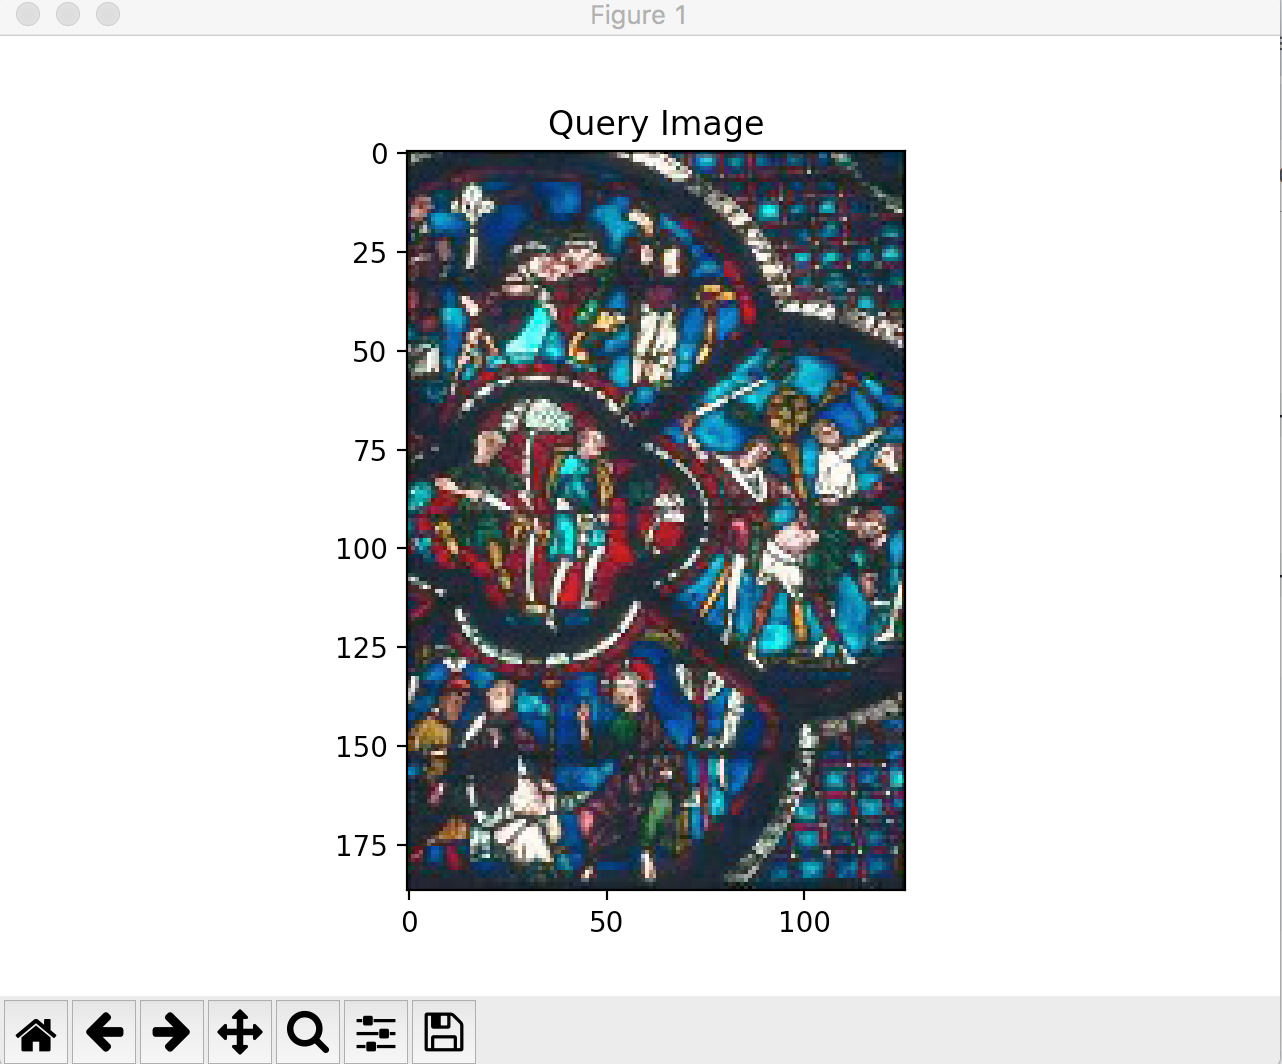
\includegraphics[width=\linewidth]{Stream1}
\caption{KNN}\label{1}  
\end{figure} 


\chapter{Discussion}
The whole program does not apply multi process, multi thread and other concurrent technology, so it runs slowly.
Comparison of SVM and CNN methods
Advantage:
 (1) Nonlinear mapping is the theoretical basis of SVM. SVM uses inner product kernel function instead of nonlinear mapping to high dimensional space.
 (2) The optimal hyperplane of feature space partition is the goal of SVM, and the idea of maximizing classification margin is the core of SVM.
 (3) support vector is the training result of SVM, and the support vector is the decisive factor in SVM classification decision.
 (4) SVM is a new small sample learning method with a solid theoretical foundation. It basically does not involve probability measure and law of large numbers, so it is different from the existing statistical methods. Essentially, it avoids the traditional process from induction to deduction to achieve efficient "transductive reasoning" from training samples to forecast samples, greatly simplifying the usual classification and regression problems.
 (5) The final decision function of SVM is determined only by a few support vectors, and the complexity of calculation depends on the number of support vectors, not the dimension of sample space, which in a sense avoids the "dimension disaster".
 (6) A few support vectors determine the final result, which not only helps us grasp the key samples and "eliminate" a large number of redundant samples, but also dooms the method not only simple algorithm, but also has a good "robustness". This "robustness" is mainly reflected in:
  1) Adding or deleting non support vector samples has no effect on the model.
  2) The support vector sample set has definite robustness.
  3) In some successful applications, the SVM method is not sensitive to the selection of nuclei.

Shortcomings:
(1) SVM algorithm is difficult to implement for large-scale training samples.
Because SVM uses quadratic programming to solve support vectors, quadratic programming involves the operation of m-order matrix (the number of samples in m) when the number of M is large, the storage and calculation of the matrix will consume a lot of machine memory and computing time. The main improvements to the above problems are the SMO algorithm of J. Platt, the SVM of T. Joachims, the PCGC of C. J. C. Burges, the C SVM of Zhang Xuecheng and the SOR algorithm of O. L. Mangasarian.
 (2) There are difficulties in using SVM to solve multiple classification problems.
The classical support vector machine algorithm only gives two classes of classification algorithm, and in the practical application of data mining, it is generally necessary to solve the problem of multi-class classification. It can be solved by combining two kinds of support vector machines. There are mainly one-to-many combination pattern, one-to-one combination pattern and SVM decision tree, and then through the construction of a combination of multiple classifiers to solve. The main principle is to overcome the inherent shortcomings of SVM, combined with the advantages of other algorithms, to solve the classification progress of multi-class classification problems.
Advantages and disadvantages of CNN convolutional neural network
Advantage
Sharing convolution kernel, no pressure on high-dimensional data processing.
It is not necessary to manually select features and train weights so that the feature classification results are good.
Shortcoming
The need to adjust parameters, large sample size, training is best to GPU
The physical meaning is not clear (that is, we do not know what features are extracted without a convolution layer, and the neural network itself is an inexplicable "black box model")




\chapter{Conclusion}

We have revisited serveral of the most established image retrieval
datasets, that were perceived as performance saturated.
To make it suitable for modern image retrieval benchmarking,
we address drawbacks of the original annotation.

This includes new annotation for both datasets that was created
with an extra attention to the reliability of the ground
truth, and an introduction of 1M hard distractor set.
An extensive evaluation provides a testbed for future
comparisons and concludes that image retrieval is still an
open problem, especially at large scale and under difficult
viewing conditions.

We present a full image indexing pipeline that exploits
supervised deep learning methods to build an inverted file as
well as a compact feature encoder. Previous methods have
either employed unsupervised inverted file mechanisms, or
employed supervision only to derive feature encoders. We
establish experimentally that our method achieves state of
the art results in large scale image retrieval.
\addcontentsline{toc}{chapter}{Reference}
\bibliographystyle{unsrt}
\bibliography{camp}
\end{document}

